\documentclass[10pt,twocolumn,letterpaper]{article}
\usepackage[T1]{fontenc}
\usepackage[utf8]{inputenc}
\usepackage{mathptmx,amsmath,amssymb,graphicx,booktabs,microtype}
\usepackage[letterpaper,left=0.70in,right=0.70in,top=0.72in,bottom=0.78in,columnsep=0.25in]{geometry}
\usepackage{titlesec}
\usepackage{balance}
\usepackage[font=footnotesize,labelsep=period]{caption}
\usepackage[hidelinks]{hyperref}
\hypersetup{pdftitle={Taxi-System Simulation and Statistical Output Analysis},pdfauthor={Roberto Mahamalimage}}
\renewcommand{\ttdefault}{pcr}
\graphicspath{{figures/}}
\renewcommand{\thesection}{\Roman{section}}
\renewcommand{\thesubsection}{\Alph{subsection}}
\renewcommand{\thetable}{\Roman{table}}
\renewcommand{\tablename}{TABLE}
\renewcommand{\figurename}{Fig.}
\captionsetup[table]{labelsep=newline}
\titleformat{\section}{\centering\normalfont\scshape}{\thesection.}{0.6em}{}
\titleformat{\subsection}{\normalfont\itshape}{\thesubsection.}{0.5em}{}
\titlespacing*{\section}{0pt}{1.3ex plus .4ex minus .2ex}{0.7ex}
\titlespacing*{\subsection}{0pt}{1ex plus .3ex minus .2ex}{0.5ex}
\setlength{\textfloatsep}{9pt plus 2pt minus 2pt}
\setlength{\floatsep}{8pt plus 2pt minus 2pt}
\setlength{\dbltextfloatsep}{10pt plus 2pt minus 2pt}
\renewcommand{\topfraction}{0.9}
\renewcommand{\dbltopfraction}{0.9}
\renewcommand{\textfraction}{0.07}
\setlength{\parindent}{1em}
\setlength{\parskip}{0pt}
\setlength{\emergencystretch}{1em}
\frenchspacing
\raggedbottom

\title{\fontsize{20}{23}\selectfont Taxi-System Simulation and Statistical Output Analysis}
\author{\normalsize Roberto Mahamalimage\\
\normalsize\textit{Politecnico di Torino}\\
\normalsize Student ID: s360997\\
\normalsize s360997@studenti.polito.it}
\date{}

\begin{document}
\maketitle

\noindent\textbf{\textit{Abstract}---This report presents two connected simulation
laboratories. The first develops a discrete-time taxi model with spatial demand,
app dispatching, taxi stands and fleet relocation, and studies daily demand and
supply shocks. The second introduces constant-input experiments, an online
warm-up detector and independent-replication confidence intervals. Rain-induced
slowdowns approximately double app waiting relative to a demand-only rain
control. Combined stress leaves a substantial backlog. In the stationary-input
baseline, mean app waiting is 6.524 minutes with a nominal 95\% interval of
[6.300, 6.747]. Longer measurements improve precision, whereas greater demand
increases both waiting and uncertainty. Assumptions, incomplete observations
and the heuristic nature of transient detection are explicitly distinguished.}

\section{Problem Overview}
The first laboratory asks for a tractable model of passenger generation,
closest-idle-taxi dispatch, trip execution, return to stands and optional fleet
rebalancing. Its purpose is to identify relevant parameters and performance
indicators and explain their effects through scenario experiments. The second
laboratory adds online detection of the end of the initial transient, reliable
output inference and a study of factors affecting accuracy.

These objectives require two different experimental settings. Daily rush hours,
scheduled arrivals and events produce \emph{non-stationary inputs}; their
24-hour outcomes are terminating-simulation results. Constant-input runs are
used separately to investigate steady-state performance. Constant inputs are
necessary for this analysis but do not guarantee stable queues.

\section{Model Design and Assumptions}
\subsection{Spatial Mobility and Service Rules}
The following assumptions define the model and delimit its interpretation.
\begin{enumerate}
\setlength{\itemsep}{1pt}\setlength{\topsep}{2pt}
\item The city is a fixed $10\times10$ km square divided into four equal zones.
Urban origins are uniform within each zone; destination zones follow a fixed
origin--destination probability matrix, followed by uniform sampling within
the destination zone. This captures spatial heterogeneity, but not directional
changes in commuting patterns.
\item Each passenger requests one vehicle, using app/phone with probability
$p_{\rm app}=0.70$ or walking to the nearest stand. Modes and destinations are
exogenous. Walking speed is constant; passengers do not abandon, switch mode
or change stand after joining. Passenger queues have no capacity limit.
\item Taxis are homogeneous, carry one passenger and serve one trip at a time.
There are no shifts, breaks, fares, fuel constraints or ride sharing, and no
separate boarding or alighting dwell time. Only taxis
parked in state \texttt{idle} are dispatchable; returning or rebalancing taxis
cannot accept app requests. App requests are processed FIFO and assigned to
the nearest idle taxi. Stand queues are also FIFO.
\item Eight ordinary stands have ten parking spaces each. The station and
airport add stands with 14 and 18 spaces. A taxi returns to the nearest stand
with currently free space; places are not reserved en route, so a taxi may be
redirected on arrival. Waiting stand passengers are served before parking.
\item Every run starts with no passengers and taxis distributed round-robin
over stands, respecting capacity. Speeds depend on prescribed conditions,
not an endogenous traffic network. All numerical values are illustrative,
without calibration to a real city.
\end{enumerate}

For positions $x,y$, the road-distance approximation and walking time are
\begin{equation}
 d(x,y)=\kappa\lVert x-y\rVert_2,\qquad
 t_{\rm walk}(x,s)=\frac{60\lVert x-s\rVert_2}{v_w},
 \label{eq:distance}
\end{equation}
where $\kappa=1.20$, $v_w=4.8$ km/h and times are in minutes. Taxis move along
straight segments, with progress scaled to the road distance. In an interval of
$h$ minutes, the road distance travelled is
\begin{equation}
 \Delta d=\min\!\left\{d_{\rm remaining},\frac{v(t,x)h}{60}\right\}.
 \label{eq:movement}
\end{equation}
The effective speed is the time-of-day baseline multiplied by weather,
transit, event and hub-congestion factors, with a floor of 6 km/h. The baseline
is 20 km/h in rush hours, 32 at night and 28 otherwise. These factors are
exogenous supply reductions rather than a traffic-flow model.
In the rain experiments, the weather factor is $\max(1-0.30r,0.40)$;
the demand-only control sets the coefficient 0.30 to zero. The transit speed
factor is $\max(1-0.18(1-a_z),0.50)$. A strike sets availability to 0.25
between 06:00 and 22:00.

\subsection{Demand and Fleet Management}
Ordinary demand in zone $z$ is approximated on the simulation grid by
independent Poisson counts:
\begin{align}
 N_z(t,t+h)&\sim\operatorname{Poisson}\!\left(\lambda_z(t)h/60\right),\label{eq:poisson}\\
 \lambda_z(t)&=\lambda_z^0 g_h(t)g_d(t)m(1+0.35r)\nonumber\\
 &\quad\times[1+(1-a_z(t))]\,e_z(t).\label{eq:rate}
\end{align}
The four base rates $\lambda_z^0$ are 5, 6, 4 and 5 passengers/hour.
$g_h$ and $g_d$ encode hour and weekday, $m$ scales urban demand, $r\in[0,1]$
is rain intensity and $a_z\in[0,1]$ is transit availability. The factor $e_z$
equals 0.70 in the event zone during the event and one otherwise.

At each scheduled hub arrival, the model samples
$L\sim\operatorname{Poisson}(\ell)$ travellers and
$N_h\mid L\sim\operatorname{Binomial}(L,q)$ taxi users. The station uses
$(\ell,q)=(70,0.08)$ and 13 daily arrivals; the airport uses $(55,0.16)$ and
nine arrivals. Their app probabilities are 0.45 and 0.60. Origins have small
Gaussian perturbations around the terminal, clipped to the city. Four percent
of ordinary urban trips target a hub when hubs are enabled.

Event demand is explicitly directional: passengers travel to the venue before
the event and leave it afterwards. For inbound volume $V_{\rm in}$, outbound
volume $V_{\rm out}$, pre-window length $L_{\rm in}$ and post-window length
$L_{\rm out}$, the per-minute rates are
\begin{align}
 \eta_{\rm in}(s)&=\frac{2V_{\rm in}s}{L_{\rm in}^2},
       &&0\leq s<L_{\rm in},\label{eq:eventin}\\
 \eta_{\rm out}(u)&=\frac{V_{\rm out}e^{-u/\tau}}
 {\tau(1-e^{-L_{\rm out}/\tau})},
       &&0\leq u<L_{\rm out}.\label{eq:eventout}
\end{align}
Counts are Poisson with mean equal to rate times step length. The tested event
lasts 20:00--22:00, with attendance 1,100, taxi shares 0.07 inbound and 0.11
outbound, $L_{\rm in}=120$, $L_{\rm out}=90$ and $\tau=28$ minutes. Local origins
or destinations are perturbed around the venue and clipped to city bounds.

Every 30 minutes, rebalancing computes desired idle counts proportional to
forecast zone demand, including upcoming hub and outbound-event requests.
At most $\lfloor0.25I(t)\rfloor$ idle taxis are moved from surplus to deficit
zones, where $I(t)$ is the number idle. This is a simple zone-level rule, not
an optimizer of the current queues at individual stands.

\subsection{Time Convention and Performance Indicators}
The nominal resolution is one minute. Generation, app dispatch and rebalancing
use the state at the beginning of each interval; taxis and walkers then advance.
Positive-duration movement completions are recorded at its end. Zero-distance
access is immediate, and the final interval is shortened to the requested
horizon. Time discretization remains a source of approximation.

Let $r_i$, $s_i$, $p_i$ and $d_i$ denote request, stand-arrival, pickup and dropoff
times. For the observed sets of app passengers already boarded ($\mathcal A_b$),
stand users who arrived ($\mathcal S_a$) and stand users boarded ($\mathcal S_b$),
\begin{align}
 \overline W_{\rm app}&=\frac{\sum_{i\in\mathcal A_b}(p_i-r_i)}{|\mathcal A_b|},\label{eq:waiting}\\
 \overline T_{\rm walk}&=\frac{\sum_{i\in\mathcal S_a}(s_i-r_i)}{|\mathcal S_a|},\qquad
 \overline W_{\rm stand}=\frac{\sum_{i\in\mathcal S_b}(p_i-s_i)}{|\mathcal S_b|}.
 \label{eq:standmetrics}
\end{align}
Total access is $p_i-r_i$, including walking for stand users. Completion and
fleet-state shares over horizon $T$, with $F$ taxis, are
\begin{equation}
 C=\frac{N_{\rm completed}}{N_{\rm generated}},\qquad
 U=\frac{\sum_f T_f^{\rm occupied}}{FT},\qquad
 A=\frac{\sum_f T_f^{\rm idle}}{FT}.\label{eq:shares}
\end{equation}
Empty-running time and empty-distance share are reported separately. Availability
$A$ is a time--fleet fraction, not the probability of immediate assignment.
Undefined means for empty populations are recorded as missing, not zero.

Daily waiting means are conditional on observed boarding, including passengers
still travelling. The model also reports backlogs and lower-bound means over
all arrivals. For the set $\mathcal A$ of all app requests observed by $T$,
\begin{equation}
 \overline L_{\rm app}(T)=\frac{1}{|\mathcal A|}
 \left[\sum_{i\in\mathcal A_b}(p_i-r_i)
       +\sum_{i\in\mathcal A\setminus\mathcal A_b}(T-r_i)\right].
 \label{eq:lowerbound}
\end{equation}
An unserved user's final waiting time is still unknown. Thus unfinished
requests are not silently treated as served or as zero-wait observations.

\section{Laboratory 1: Daily Scenario Results}
Seven 24-hour scenarios were run with $F=40$ and five replications each, using
seeds 1000--1004. The baseline is Wednesday with hubs and rebalancing enabled.
The scenarios change hub presence, rain, transit service or the evening event;
combined stress also uses Friday demand. All tables average per-replication
statistics, rather than pooling passengers across runs.

\begin{table}[tb]
\centering
\caption{Daily results: means over five replications. Times are minutes.}
\label{tab:daily}
\setlength{\tabcolsep}{3.2pt}
\small
\begin{tabular}{lrrrr}
\toprule
Scenario & App wait & Walk & Stand wait & $C$ (\%)\\
\midrule
Baseline & 6.08 & 12.08 & 22.56 & 98.8\\
No hubs & 5.11 & 18.65 & 2.81 & 99.0\\
Rain: demand only & 6.52 & 12.36 & 32.24 & 98.1\\
Rain: full effect & 13.35 & 12.36 & 37.55 & 97.7\\
Transit strike & 12.73 & 13.54 & 22.22 & 98.9\\
Evening event & 11.07 & 13.06 & 25.70 & 96.8\\
Combined stress & 151.13 & 15.23 & 28.16 & 71.9\\
\bottomrule
\end{tabular}
\end{table}

\begin{figure}[tb]
\centering
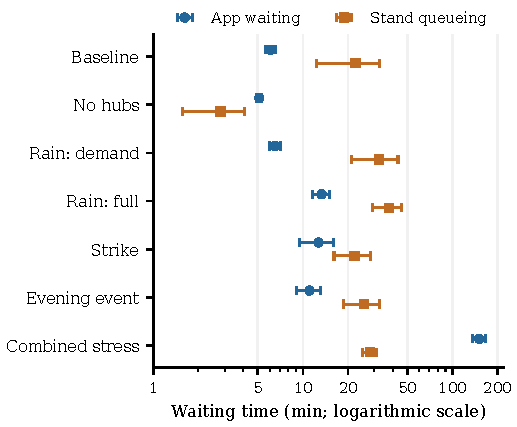
\includegraphics[width=\columnwidth]{lab1_waiting.pdf}
\caption{Daily waiting means with sample standard deviations across five runs.
The bars are descriptive variability, not confidence intervals. Waiting is
conditional on boarding; the logarithmic axis keeps combined stress visible.}
\label{fig:daily}
\end{figure}

Table~\ref{tab:daily} and Fig.~\ref{fig:daily} show that demand and effective
supply must be considered together. The two rain scenarios generate exactly
the same requests for matched seeds: their mean demand is 789 users/day.
Adding the weather speed penalty increases app waiting from 6.515 to 13.352
minutes, approximately 105\%, and lowers the idle share from 65.1\% to 50.3\%.
This comparison isolates the additional effect of slower circulation; the
baseline generates only 619.8 users/day.

The event produces an average 198.4 event requests and reduces completion to
96.8\%. Combined stress generates 1,433.4 requests, with average counts of
353.0 app users not yet boarded, 28.6 stand users not yet boarded and 21.4
passengers still travelling at midnight. The 71.9\% completion rate therefore
does not imply that the other requests were abandoned. Its 151.131-minute
boarded-app mean is complemented by an all-app-arrival lower-bound mean of
158.315 minutes, exposing the unresolved backlog.

Baseline occupied and idle shares are 16.3\% and 71.6\%; under combined stress
they become 42.1\% and 24.5\%. Residual idle time can coexist with long queues
because of spatial mismatch, varying load and the restriction that returning
taxis are unavailable. Stand delays can likewise remain high when other
stands contain idle taxis.

The no-hub comparison changes demand, stand locations, total parking capacity
(112 versus 80), initial taxi positions, some destinations and local congestion.
It compares two configurations, not the isolated causal effect of arrival
bursts. Its longer walking mean also reflects the absence of short terminal
walks. With only five runs, these daily experiments are descriptive and do not
establish precise steady-state effects or real-city predictions.

\section{Laboratory 2: Stationary Output Analysis}
\subsection{Constant-Input Experiments}
The stationary mode fixes $g_h=g_d=1$ and the base taxi speed at 28 km/h.
Hubs, events, temporary disruptions and periodic rebalancing are disabled.
Baseline urban demand is consequently 20 users/hour, with $F=20$, eight stands
and the same spatial rules as before. Rain is zero and transit availability one.
This is a different configuration from Laboratory~1, not a warm-up correction
applied to its non-stationary daily scenarios.

\subsection{Online Transient Detection}
The monitored state is $X(t)=(Q(t),U_{\rm inst}(t),G(t))$: the number of
not-yet-boarded users including walkers, the instantaneous occupied fleet
fraction, and the mean age of those pending requests (zero if none).
Monitoring current state, rather than cumulative performance averages, helps
expose persistent growth or starvation.

Non-overlapping 30-minute, time-weighted batch averages feed a bounded-memory
detector. On the latest $2w$ batches ($w=12$), let $\bar X_j^-$ and $\bar X_j^+$
be the means of the older and newer windows, $s_j$ the sample standard
deviation across both, and $\hat\beta_j$ the least-squares slope against batch
index. For each component,
\begin{align}
 S_j&=a_j+0.5s_j,\qquad
 D_j=\frac{|\bar X_j^+-\bar X_j^-|}{S_j},\label{eq:detector}\\
 L_j&=\frac{|\hat\beta_j|(2w-1)}{2S_j}.\label{eq:drift}
\end{align}
The absolute tolerances are $a=(1.5,0.05,5)$ in users, fleet fraction and
minutes. A check passes if $D_j\leq1$ and $L_j\leq1$ for every component.
Three consecutive passes trigger a decision; the earliest possible decision
is 13 simulated hours. Only already observed data are used. These thresholds
are practical tolerances, not significance levels or a formal stationarity test.

Three independent pilot runs determine the common deletion time
$B=\max_{k=1,2,3}\hat B_k$. If any pilot fails to detect stability within 96
hours, the configuration is marked as undetected and receives no steady-state
interval. Fig.~\ref{fig:warmup} contrasts a representative
baseline trajectory with persistent growth under overload. Non-detection
alone is not a mathematical proof of instability.

\begin{figure}[tb]
\centering
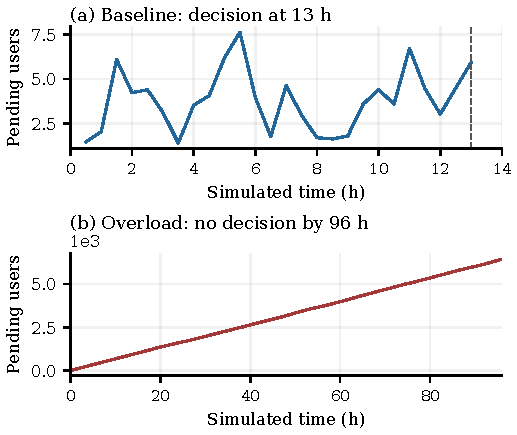
\includegraphics[width=\columnwidth]{warmup_traces.pdf}
\caption{Pending-user batch averages from pilot 0 (seed 3481032016).
The baseline pilot stops at its 13-hour decision. Under overload, pending
users continue accumulating throughout the 96-hour screening horizon.}
\label{fig:warmup}
\end{figure}

\begin{figure*}[t]
\centering
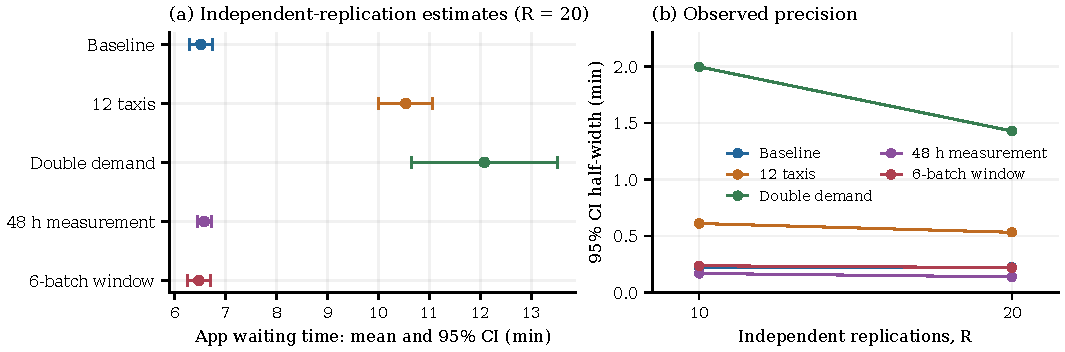
\includegraphics[width=\textwidth]{precision_comparison.pdf}
\caption{Stationary-input app waiting. (a) Nominal 95\% Student-$t$ intervals
across 20 independent production replications. (b) CI half-width for two
predeclared sample sizes, using the same replication prefix. Configurations
without detected stability are excluded from interval estimation, not silently
counted as successful runs.}
\label{fig:precision}
\end{figure*}

\subsection{Independent Replications and Confidence Intervals}
Production uses new random streams, independent of the pilots. Each of $R=20$
replications starts from the prescribed empty state, discards the same $B$ and
measures a fixed $H=24$ hours. Separating pilot selection from production avoids
choosing the deletion time from the observations used for inference~\cite{law}.

For waiting metrics, the cohort contains every arrival in $[B,B+H)$. Normal
arrivals continue while this cohort is followed to pickup, for at most another
48 hours. Stopping new arrivals would change the service environment. A
timeout invalidates the measurement; failed replications are not dropped to
manufacture an interval. No such timeout occurred in the reported production
runs. Fleet shares use counter differences over $[B,B+H)$ only, excluding
follow-up time.

\begin{samepage}
Let $Y_r$ be one replication's mean for a specified KPI. With $\bar Y$ the
average across replications and $s_Y$ their sample standard deviation,
\begin{align}
 \bar Y&=\frac1R\sum_{r=1}^R Y_r,\qquad
 s_Y^2=\frac{\sum_{r=1}^R(Y_r-\bar Y)^2}{R-1},\label{eq:repstats}\\
 \operatorname{CI}_{1-\alpha}&=\left[\bar Y-h_R,\bar Y+h_R\right],\quad
 h_R=t_{1-\alpha/2,R-1}\frac{s_Y}{\sqrt R}.\label{eq:ci}
\end{align}
\end{samepage}
Student's critical value~\cite{student} is used with $\alpha=0.05$. The sample
size and observation duration are fixed before production; the first ten and
all twenty replications form two predeclared precision comparisons. Individual
minutes or passenger waits are not treated as independent samples, since queueing
induces serial dependence. The interval is approximate for replication means
and remains sensitive to residual initial bias and non-normality.

The estimand is the expected per-replication window mean, approximating a
steady-state KPI when deletion is adequate. It is not a pooled mean across all
customers, an individual passenger prediction interval, or a simultaneous
95\% statement about every configuration. Seeds are reused across
configurations, but no paired-difference intervals are claimed.

\section{Accuracy and Parameter Sensitivity}
Accuracy involves both variance and initial-condition bias:
\begin{equation}
 \operatorname{MSE}(\bar Y)=\operatorname{Var}(\bar Y)
             +\operatorname{Bias}(\bar Y)^2.\label{eq:mse}
\end{equation}
The exact taxi steady-state mean is unknown, so interval widths measure
precision directly, while deletion sensitivity probes potential bias without
quantifying it exactly. Reference-model coverage is checked separately.

\begin{table}[tb]
\centering
\caption{Stationary study design and observed common deletion time $B$.}
\label{tab:design}
\small\setlength{\tabcolsep}{4pt}
\begin{tabular}{lrrrrr}
\toprule
Configuration & $F$ & $m$ & $H$ (h) & $w$ & $B$ (h)\\
\midrule
Baseline & 20 & 1 & 24 & 12 & 13.0\\
Fewer taxis & 12 & 1 & 24 & 12 & 15.0\\
Higher demand & 20 & 2 & 24 & 12 & 19.0\\
Longer measurement & 20 & 1 & 48 & 12 & 13.0\\
Shorter window & 20 & 1 & 24 & 6 & 14.5\\
Overload & 4 & 4 & 24 & 12 & ---\\
\bottomrule
\end{tabular}
\end{table}



The five screened configurations yielded 100 complete production replications;
all three overload pilots failed screening. The baseline app-wait estimate is
6.524 minutes, with CI [6.300, 6.747]. Mean total access is 14.612 minutes
[13.676, 15.548], while occupied share is 0.2257 [0.2215, 0.2299]. Table~\ref{tab:design}
and Fig.~\ref{fig:precision} address accuracy through the following changes.

\textit{Fleet and demand.} Reducing the fleet from 20 to 12 raises estimated
app waiting to 10.539 minutes [10.008, 11.071]. Doubling demand to 40 users/hour
with 20 taxis raises it to 12.079 [10.651, 13.508]. The app-wait relative
half-width $h_R/|\bar Y|$ rises from 3.4\% in the baseline to 5.0\% and 11.8\%,
respectively. Thus increased load affects precision as well as service level:
the same replication budget gives less precise estimates in the more variable
high-demand system. Its deletion time also increases from 13 to 19 hours.

\textit{Measurement duration.} Extending useful observation from 24 to 48 hours
reduces the app-wait half-width from 0.223 to 0.137 minutes, approximately
38.7\%. The corresponding estimate, 6.592 [6.455, 6.729], is compatible with the
baseline interval. Total-access half-width also falls, from 0.936 to 0.557
minutes. Longer windows improve averaging here but cannot, by themselves,
prove the absence of residual initial bias.

\textit{Replication count.} At fixed variance, Eq.~\eqref{eq:ci} suggests an
approximately $R^{-1/2}$ reduction in uncertainty. In the higher-demand case,
increasing $R$ from ten to twenty reduces half-width from 1.996 to 1.428
minutes. The baseline instead changes slightly from 0.218 to 0.223: its
estimated between-replication standard deviation increases from 0.305 to 0.477.
The expected precision trend is not a guarantee of monotonic improvement in
one realized sample. There is no adaptive stopping at a desired interval width.

\textit{Detector window.} With $w=6$, the first pilot decides at seven hours,
but the conservative maximum across pilots is 14.5 hours, versus 13 with
$w=12$. Shorter windows therefore need not shorten the final deletion time.
The app estimate becomes 6.485 [6.266, 6.704]. Agreement is a useful sensitivity
check, not proof that both deletions remove all initial bias.

\subsection{Coverage Check on a Known Queue}
Inference is additionally checked on an M/M/1 queue with $\lambda=0.5$ and
$\mu=1$. Its theoretical mean queueing wait is
\begin{equation}
 \mathbb E[W_q]=\frac{\lambda}{\mu(\mu-\lambda)}=1.\label{eq:mm1}
\end{equation}
Workload is initialized from its exact invariant distribution: zero with
probability $1-\rho$, otherwise exponential with rate $\mu-\lambda$, where
$\rho=\lambda/\mu$. Subsequent waits obey Lindley's recursion
$W_{n+1}=\max\{0,W_n+S_n-A_n\}$ with independent exponential service and
interarrival times. This preserves within-replication dependence while removing
initial bias from this particular reference test.

Across 300 experiments, each with 20 independent replications of 3,000
customers, 283 nominal 95\% intervals contain the true mean: empirical coverage
is 94.3\%. Its 95\% Wilson binomial interval is [91.1\%, 96.4\%], consistent with
the nominal target. The grand mean is 1.0016. This checks the interval method
on a solvable dependent-output model; it does not establish coverage for taxi
intervals or validate the warm-up heuristic itself.

\balance
\section{Verification, Limitations and Conclusions}
All 39 automated tests passed. They cover chronological consistency, known
trip distances, parking limits, zero relocation, horizon truncation, transient
and drifting test signals, a known Student-$t$ interval, stream separation and
cohort follow-up. Numerical summaries were cross-checked against the archived
replication CSV files. The implementation uses Python 3.12.14, NumPy 2.3.5,
pandas 2.2.3 and SciPy 1.17.0. Daily seeds are 1000--1004; the stationary study
uses root seed 20261025 and separate pilot/production seed families. The M/M/1
coverage experiment uses seed 71023.

The main limitations are illustrative spatial and demand assumptions,
exogenous congestion, one-minute discretization and a basic zone-level
relocation policy. Finite-window stability screening can accept a temporary
plateau or miss a slow transient; it cannot prove steady state. Intervals
quantify sampling precision under the experimental design, not calibration
error, discretization bias or model realism. The daily study likewise retains
its explicit finite-horizon interpretation and observed backlogs.

Together, the laboratories demonstrate how demand shocks and slower supply
create queueing pressure, and why credible output analysis needs more than a
single run. Independent production, explicit cohort observation and reported
screening failures make uncertainty visible. Longer measurements improve
precision in the tested case, while heavier load demands a larger statistical
budget. Sensitivity to warm-up settings must accompany narrow intervals.

\begin{thebibliography}{2}
\setlength{\itemsep}{0pt}
\bibitem{law} A. M. Law, \textit{Simulation Modeling and Analysis}, 5th ed.
McGraw-Hill Education, 2015.
\bibitem{student} Student, ``The probable error of a mean,'' \textit{Biometrika},
vol. 6, no. 1, pp. 1--25, 1908.
\end{thebibliography}
\end{document}
